\chapter{Intensity Integration}

\section{The Integration Algorithm}\label{integration_algorithm}

An intensity integration is a plot of average intensity as 
a function either $Q$, $2\theta$, or $\chi$. The calibration 
values for the diffraction data must be known before 
the integration is done. A range and bin size for the
integration must be give. For example, a $Q-I$ integration 
might have a range from 2 to 5 with 100 bins. 

The algorithm for performing the intensity integration
is as follows: loop over every pixel in the image. 
Add its intensity to a bin if it $Q$, $2\theta$, 
or $\chi$ value falls within the bin's range.
We need to know the calibration values because
they are used to calculate $Q$, $2\theta$ and $\chi$
from the pixel's coordinates using 
using equations~\ref{ytermsydoubleprime}
\ref{xtermsxdoubleprime}, \ref{chitermsyx}, 
\ref{2thetatermsr}, and \ref{qterms2theta}.
After binning all the pixel, the bins are then averaged.

This program can constrain the integration range. 
This means that you can perform, for example,
a $Q$ integration of only those pixels with some
particular $\chi$ range. Or, you can
constrain your $\chi$ integration to a particular
$Q$ range. This could be used, for example, to
perform a $\chi$ integration of only one
diffraction peak. The algorithm for performing
the constraint isn't different. You just
only bin intensity values which are allowed by 
by the constraint.

The program can perform a polarization 
correction to the integration. The polarization 
correction formula is
\begin{align}
    I&=Im/PF \\ 
    PF&=P(1 - (\sin(2\theta)\sin(\chi-90))^2) + 
    (1 - P)(1 - (\sin(2\theta)\cos(\chi-90))^2)
\end{align}
with $Im$ the measured intensity.  The $2\theta$ 
and $\chi$ values correspond to the particular 
value that is being corrected. If this option
is selected, all pixels have their intensity
corrected by this formula before they
are binned. 

\section{Integrating with the Program}

The program requires one or more diffraction images and
calibration parameters to be loaded into the program
before an intensity integration can be done.
Figure~\ref{integration_tab} shows the
\gui{Integrate} tab. This is where integration is done.
There are two sets of inputs on the tab. 
The inputs on the left is titled \gui{Q-I Integration}
and can be used for performing $Q$ integration.
The \gui{Q Lower?} and \gui{Q Upper?} inputs on the left 
can be used to specify an integration range in $Q$.
The number of bins in $Q$ space can be specified with the
\gui{Number of Q?} input. The \gui{Integrate} button
on the left can be used to perform a $Q$ integration.

\begin{SCfigure}[1][htbp]
    \centering
    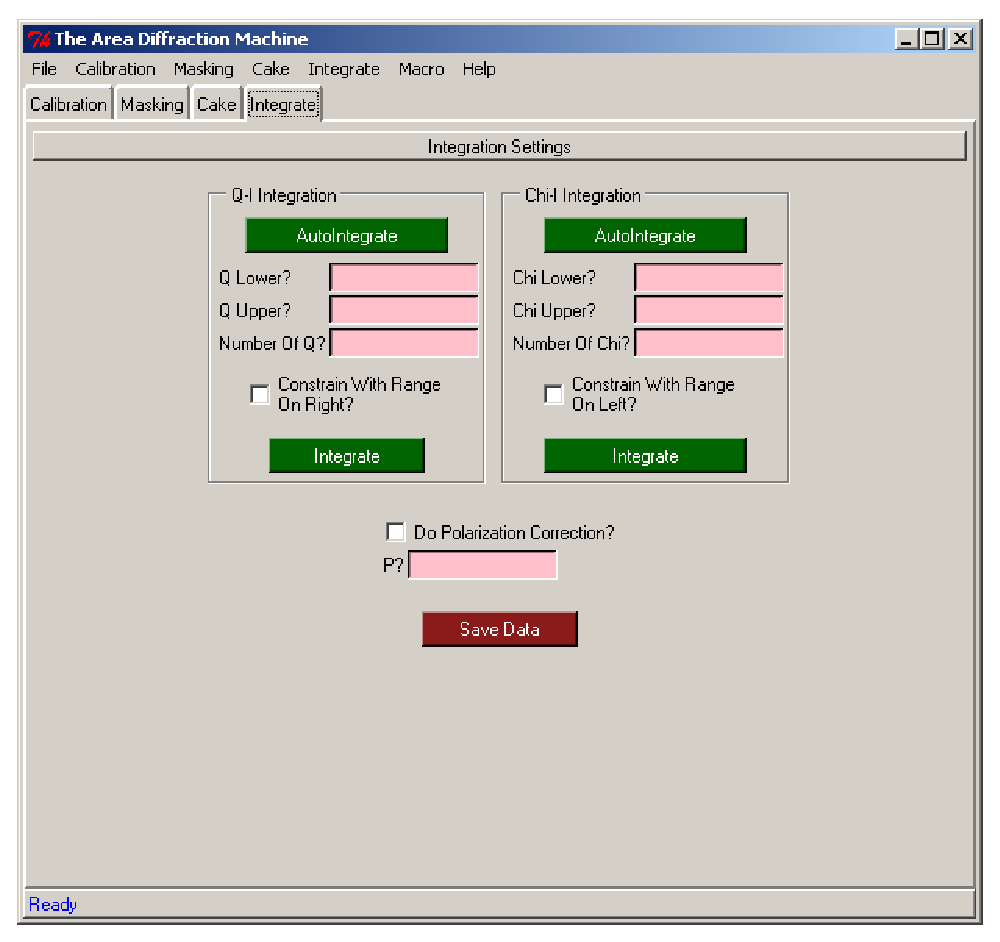
\includegraphics[scale=.75]{figures/integration_tab.eps}
    \caption{The integration tab. This is where intensity
    integration is done.} 
    \label{integration_tab}
\end{SCfigure}

The inputs on the right is titled \gui{Chi-I Integration}
and can be used for performing a $\chi$ integration.
The \gui{Q Lower?} and \gui{Q Upper?} inputs on the right
can be used to specify an integration range in $\chi$.
The number of bins in $\chi$ space can be specified with the
\gui{Number of Chi?} input. The \gui{Integrate} button
on the right can be used to perform $\chi$ integration.

\section{The Integration Window}

\begin{SCfigure}[1][htbp]
    \centering
    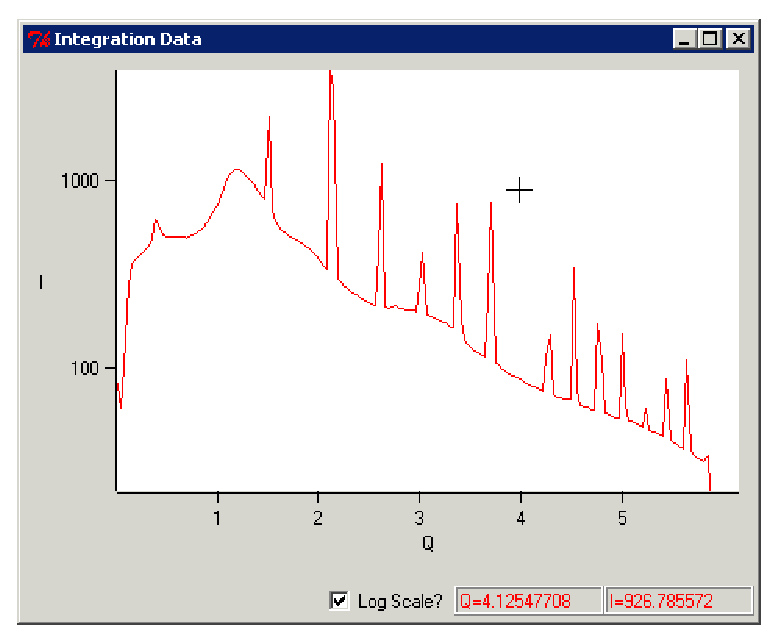
\includegraphics[scale=.75]{figures/integration_window_q.eps}
    \caption{The integration window that
    opens up after an intensity integration 
    is performed.} 
    \label{integration_window_q}
\end{SCfigure}

\begin{SCfigure}[1][htbp]
    \centering
    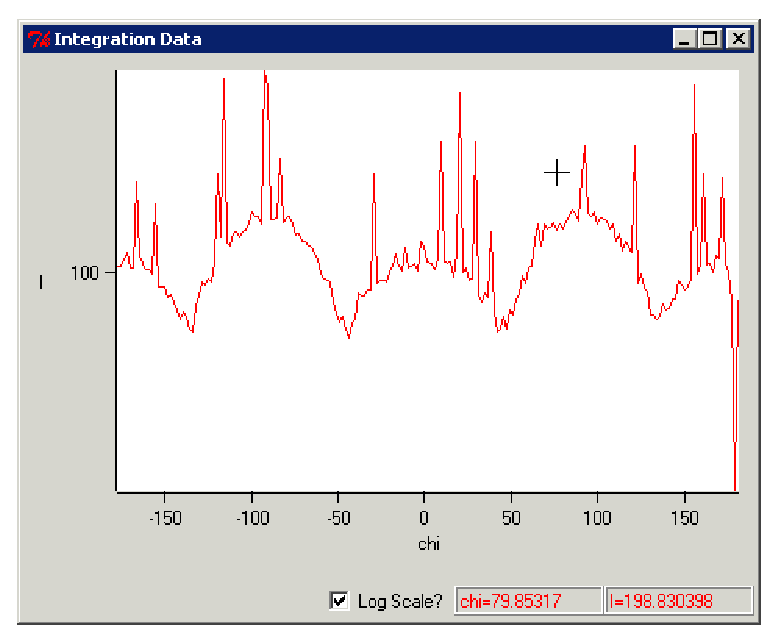
\includegraphics[scale=.75]{figures/integration_window_chi.eps}
    \caption{The integration window that opens up after 
    you perform an intensity integration.} 
    \label{integration_window_chi}
\end{SCfigure}

After the program finishes integrating, a line plot
of the integrated data will be displayed in a new window. 
Figure~\ref{integration_window_q} shows 
the integration window displaying $Q-I$ integrated data
and figure~\ref{integration_window_chi} shows the
window displaying $\chi-I$ integrated data.
This window has a couple of nice features for interacting
with the data:
\begin{itemize}
    \item {\em Zoom into the data} -- left click on the plot and 
    hold down on the mouse. When the mouse is moved around, the
    program will create a resizing rectangle.  When the mouse is 
    released, the program will zoom into the selected range.
    \item {\em Zoom out of the data} -- right
    click on the plot.
    \item {\em Resize the window} -- click on the bottom right 
    corner of the window and drag. The window will resize just 
    like any other window and the plot will become larger or 
    smaller.  
    \item {\em Read coordinates for a selected point} --
    when mousing over certain the plot, the selected $Q$, $\chi$
    or $2\theta$ and intensity value will be displayed on
    the bottom of the window.
    \item {\em Log Scaling} -- the \gui{Log Scale?} check box
    will toggle whether to display a log scale of the data.
\end{itemize}

\section{\texorpdfstring{Working in $2\theta$}{Working in 2theta}}

This program can integrate in $2\theta$ instead of $Q$. This
The \gui{Work in 2theta} option in the menu bar can be used
to change the way that integration is done. This option will
make the label on the left to say 
\gui{$2\theta$-I Integration}. The inputs below will 
change to \gui{$2\theta$ Lower}, \gui{$2\theta$ Upper}, 
and \gui{Number of $2\theta$}. The 
\gui{Integrate} button will then perform an integrate 
in $2\theta$. The diffraction window will display
average intensity as a function of $2\theta$.
If there are any values in the \gui{Q Lower} or
\gui{Q Upper}, they will be convert from $Q$ to $2\theta$
values when the program switches. The \gui{Work in Q} option
in the menu bar can be used to change the program 
back to working with $Q$. Any values in the \gui{$2\theta$ Lower?}
or \gui{$2\theta$ Upper?} will be converted back.

\section{AutoIntegrate}

There is a convenience function called \gui{AutoIntegrate} 
that is similar to the \gui{AutoCake} button.
\gui{AutoIntegrate} will try to pick a nice integration range 
and then do the integration. The AutoIntegrate button 
on the left will guess at a nice range of $Q$ 
(or $2\theta$) and then do the $Q$ (or
$2\theta$) integration.
It will always make the lower $Q$ or $2\theta$ 
value 0 and the upper value large enough
to include all the data.
It will set the number of $Q$ or $2\theta$ to
200. The \gui{AutoIntegrate} button on the right 
will guess a nice range of $\chi$ and 
do the $\chi$ integration. It will always 
set \gui{Chi Lower} to -180, \gui{Chi Upper} to
180, and \gui{Number of Chi} to 200.

\section{Constraining the Inputs}

As was described in 
section~\ref{integration_algorithm}, an integration 
of one parameter can be constrained by another 
parameter. For example, a $Q$ or $2\theta$ 
integration can be done only of values in a 
particular $\chi$ range. $\chi$ integration 
can only be done of a particular $Q$ or $2\theta$ 
range. Of course, it would be pointless to 
constrain $Q$ to a certain range of $2\theta$
or vice versa.

To constrain the integration using the program,
there are two convenient 
\gui{Constrain With Range On Right?} and 
\gui{Constrain With Range On Left?} check boxes.

When \gui{Constrain With Range On Right?} is
selected,
the $Q$ or $2\theta$ integration being done
will be constrained in $\chi$ by the chi
range specified by \gui{Chi Lower} and 
\gui{Chi Upper}. When 
\gui{Constrain With Range On Left?} is selected, 
the $\chi$ integration will be constrained by
either the $Q$ range specified by \gui{Q Lower?}
and \gui{Q Upper?} or the $2\theta$ range specified by 
\gui{$2\theta$ Lower?} and \gui{$2\theta$ Upper?}.

\section{Masking}

The program allows for masking of certain
pixels while integrating. Masking of intensity 
integrated data is done whenever the
\gui{Do Greater Than Mask?}, \gui{Do Less Than Mask?},
or \gui{Do Polygon Mask?} check boxes are selected.
Whenever the program finds an intensity value
that should should be masked (either because it 
is too large, too small, or in a polygon mask), the
program will ignore the pixel and not bin it.
Refer to Chapter \ref{pixel_masking} for a discussion
of masking.

\section{Saving Integrated Data}

The intensity integrated data can be saved to a file
using the \gui{Save Data} button. 
A typical integration file looks like:
\begin{lstlisting}[caption={'A Cake Data File'}]
# Q vs I Intensity Integration
# Intensity integration of: C:/data/LaB6_14_02_56.mar3450 
# Data Integrated on Fri Mar 21 17:59:16 2008
# Calibration data used:
#   x center:    1725.0000000 pixels
#   y center:    1725.0000000 pixels
#   distance:     125.2960000 mm
#   energy:     12735.3957721 eV
#   alpha:          0.0000000 degrees
#   beta:           0.0000000 degrees
#   rotation:       0.0000000 degrees
#   pixel length:     100.0000000 microns
#   pixel height:     100.0000000 microns
# A polarization correction was applied
#   P = 1.000000
# A greater than mask was applied
#   Greater than mask = 10000.000000 (All pixels above 10000.000000 were ignored)
# A Less Than Mask was applied.
#   Less than mask = 50.000000 (All pixels below 50.000000 were ignored)
# Polygon mask(s) were applied
# Polygon(s) used in the analysis:
#   647.844364937	1369.72808587
#   1449.93738819	3226.88193202
#   2535.84794275	1449.93738819
#
#   1258.66905188	641.674418605
#   1215.47942755	999.531305903
#   1505.46690519	1116.76028623
#   1653.54561717	777.413237925
# Integration performed with a chi constraint
#   chi constraint lower: 90.000000
#   chi constraint upper: 270.000000
# Integration Range:
#   Q Lower = 0.000000
#   Q Upper = 6.726544
#   Number of Q = 200.000000
#   Q Step = 0.033633
# Q	Avg Intensity
0.016901	0.000000
0.050703	0.000000
0.084504	0.000000
0.118306	0.000000
0.152108	0.000000
0.185910	0.000000
...
\end{lstlisting}
The header is a bunch of lines that begin with \#.
The header describes the state that the program was
in when the intensity integration was performed.
The fist line describes what type of integration was
performed. For example, if a $\chi-I$ integration was 
performed, the header file will say
\macroline{\# Chi vs I Intensity Integration}.
The header then contains the name(s) of the diffraction
files that were integrated. The header contains the
calibration parameters that were used when integrating.
The header contains information about any polarization
correction, greater or less than mask that was applied,
polygon mask that was applied. It describes any constrains 
on the integration and finally the integration range and 
step size.  Following the header is the line
\macroline{\# Q Avg Intensity} (or \macroline{\# Chi Avg Intensity}
or \macroline{\# 2theta	Avg Intensity}). Following it is
the data. Each line contains two numbers corresponding to one bins. 
The first number is the middle $Q$ (or $\chi$ or $2\theta$ value) 
in the bin and the second number is the average intensity.
